\section{APR}
\subsection{APR 是什么}
首先请看官方说明。没看过的同学,请务必逐字逐句阅读完毕,因为APR重要性相当于一次小答辩 

\url{https://www.liverpool.ac.uk/student-administration/research-students/progression/annual-progress/}

在我的理解里,APR的作用是
\begin{itemize}
    \item Interview: 读PhD本身很不容易,所以学校、学院需要了解学生遇到的问题,帮助解决
    \item Seminar: 锻炼作报告的能力 + 认识其他博士生同学
    \item Progress report: 了解学生进度,进一步发现并帮助解决学生遇到的问题。同时,筛查完全不认真学习的学生
\end{itemize}

有同学一开始面对APR的时候会很紧张,因为如果APR不通过,直接会被退学。但实际上APR主要是帮助大家解决问题的,只要你不是确实主观上不愿意读,一年以来几乎没做事情,一般都不会不通过。所以,反而应该大胆的在APR里暴露自己的问题,寻求帮助。

\subsection{APR 流程}
\subsubsection{准备工作}
APR的前置任务只有一个,那就是要填完\textbf{每月至少一次}的会议记录。关于如何填写会议记录,参见章节 \ref{section:meeting_record}。

每年关于APR有两封重要邮件
\begin{enumerate}
    \item 
        \begin{minipage}{0.3\textwidth}
            其一为西浦在5月发的邮件,大概长这样,发到西浦邮箱
        \end{minipage}
        \begin{minipage}{0.63\textwidth}
            \begin{figure}[H]
                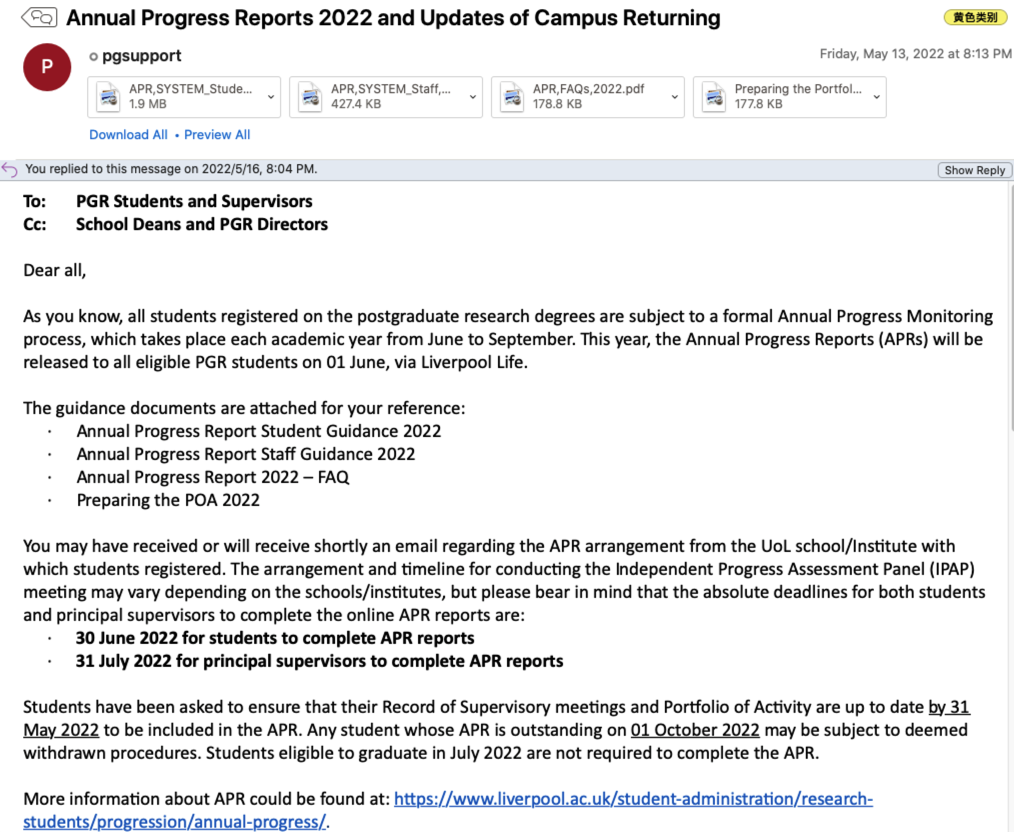
\includegraphics[width=0.95\columnwidth, right]{author-folder/Kai.Wu/APR_email.png}
            \end{figure}
        \end{minipage}

    \item 
        \begin{minipage}{0.3\textwidth}
            其二为你的利物浦学院在5月发的邮件,数学学院的大概长这样,发到利物浦邮箱。其他学院的可能不太一样
        \end{minipage}
        \begin{minipage}{0.63\textwidth}
            \begin{figure}[H]
                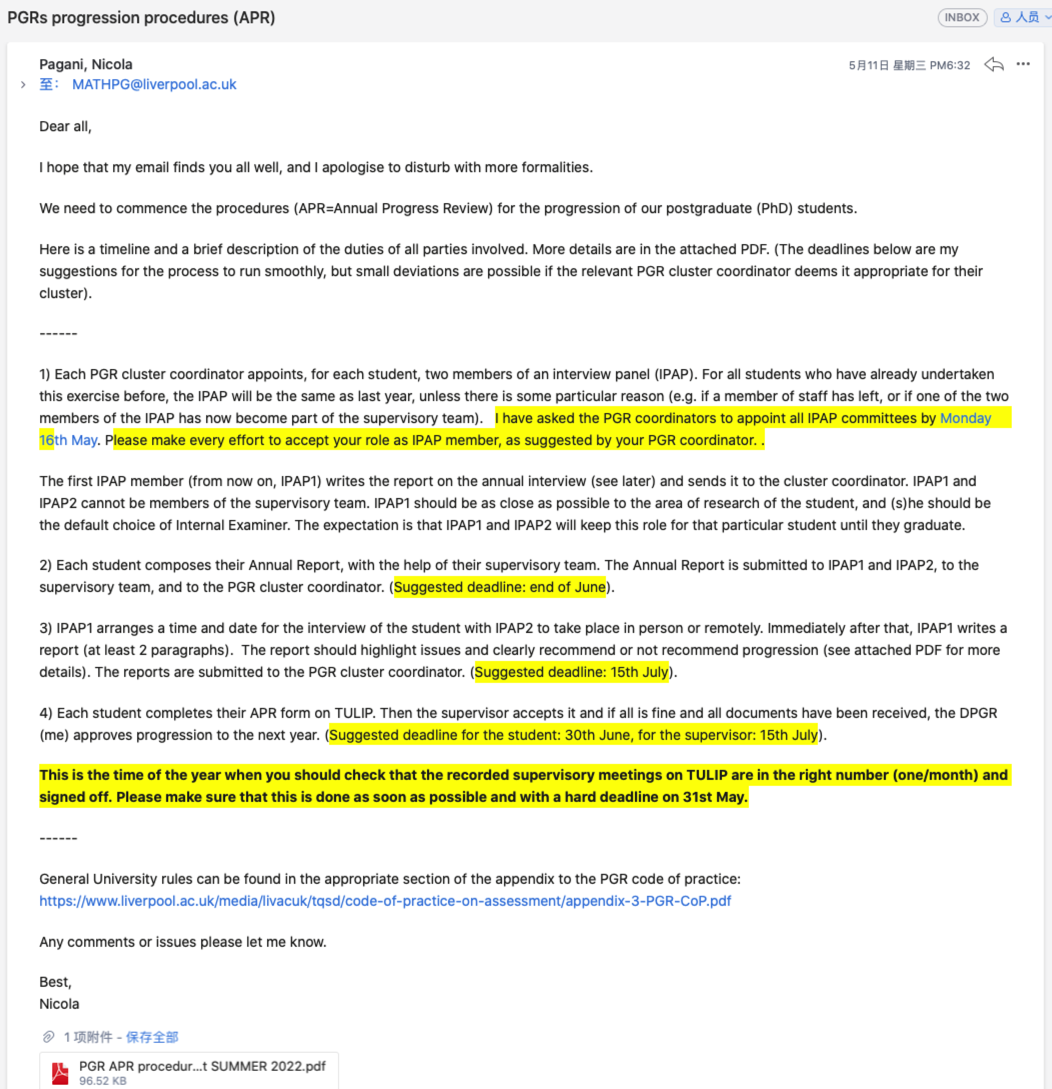
\includegraphics[width=0.95\columnwidth, right]{author-folder/Kai.Wu/APR_liverpool_email.png}
            \end{figure}
        \end{minipage}

\end{enumerate}

每个学院的APR要求略有区别,所以在5月左右,请务必查收你的利物浦邮箱。两封邮件,特别是新生,请务必仔细阅读,特别是附件内容,\textbf{初次做APR建议对两封邮件和附件,逐字阅读}。

APR的具体内容就是下面三个部分
\subsubsection{Annual Report (AR) 年度进度报告}
简单来说,把你做了什么\textbf{写成一篇文档}。一般会有字数或者页数要求。如果你不知道些什么,我个人建议可以事无巨细的写,甚至可以写流水账。比如,读了什么文献,有了什么收获;写了什么代码/做了什么实验。以及很重要的,参加了什么学术活动,比如参加conference, meeting,还有做学校的TA,都可以写进去。
\subsubsection{Annual Seminar 年度研讨会}
一般是把一个学院或者一个系的所有PhD拉到一起做个展示,互相提提意见,了解下。但据我所知,有的人少的系和学院直接跳过了这一部分,或者把这一部分融合到下面的面试里,变成给两位老师讲。不管是什么形式,你需要\textbf{做一个PPT},让别人了解你的研究。
\subsubsection{IPAP Interview 面试}
学院会找两位不是你的导师且和你没有利益冲突的老师来和你面谈。你可能需要\textbf{做一个PPT},在里面放心大胆写下你遇到的问题。由于你的导师团队被禁止接触这一部分,所以你可以畅所欲言,以下问题都可以写。按照要求,两位老师会竭尽所能帮你解决问题
\begin{itemize}
    \item 设备问题:学校电脑故障,比如哪里用起来不顺手,卡顿,死机;办公室环境问题(例如空调对着头吹)
    \item 实实在在的科研问题:你文献读得太少,但又不知道怎么高效读;你不知道实验方法;你写作有很大困难;你因为非主观的原因无法参加很多学术会议(比如这几年,每年APR我们都要吐槽疫情的各种影响)等等
    \item 导师问题:你导师压榨你,每天让你996工作,让你疲惫不堪;你导师让你做很多无关工作,比如给他搬家,给他拿外卖,给他报销;你导师对你很凶,对你很push,让你每天精神高度紧张;你导师频繁在非工作时间打电话、发微信、邮件并要求你立即回复,让你无法休息;你导师抢你论文一作;你导师长期失联,动不动就三五天不回你邮件。这些问题,其实都是导师的严重失职。一旦遇到,都可能造成很严重的心理负担,并影响后面的工作效率。IPAP就是来做这个的,请务必和面试的老师聊清楚。
    \item 情绪、心理问题:焦虑、紧张、失眠、抑郁倾向
    \item 家庭压力:你家里要求你3年毕业,但是你觉得压力太大
    \item 经济问题,身体问题(哪里严重不舒服,可能需要休学/请假休养),等等任何影响你正常PhD工作的问题
\end{itemize}

\vspace{5mm}
定位并解决所有问题,然后开启下一学年的学习,就是APR的主要目的。如果有任何APR不方便/无法解决的问题,请及时与导师、系主任、院长、你的DA、学校的免费心理咨询室沟通。


\begin{flushright}
(2022年10月12日 by Kai Wu)
\end{flushright}